\section{視線速度}

太陽系外惑星は、惑星の公転による恒星の視線速度方向の変化を、恒星スペクトルのドップラーシフトを通じて検出することで初検出された。

\begin{figure}[]
 \begin{center}
	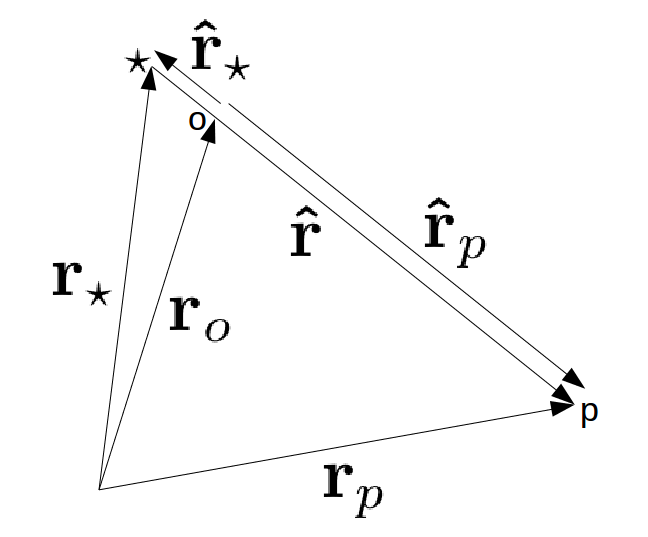
\includegraphics[bb=0 0 648 537,width=1.0\linewidth]{fig/rvector.png}
\end{center}
	\caption{重心$o$と各ベクトルの定義。\label{fig:rvector}}
\end{figure} 

惑星による恒星の視線速度変動を考える。二体の場合、恒星の視線速度は恒星と惑星の重心から測ったベクトルの運動の視線速度が観測される。そこで、図\ref{fig:rvector}のように惑星$p$、恒星$\star$とその重心$o$をおく。主星、惑星質量をそれぞれ$M_\star$、$M_p$とし、主星と惑星の位置を${\bf r}_\star$, ${\bf r}_p$とする。この系の重心${\bf r}_o$は
\begin{eqnarray}
{\bf r}_o = \frac{M_\star {\bf r}_\star+ M_p {\bf r}_p}{M_\star + M_p}
\label{eq:rbary}
\end{eqnarray}
である。重心から測った主星と惑星の位置${\bf \hat{r}}_\star = {\bf r}_\star - {\bf r}_o$, ${\bf \hat{r}}_p = {\bf r}_p - {\bf r}_o$、また主星から惑星に向かうベクトルを${\bf \hat{r}} = {\bf \hat{r}}_p - {\bf \hat{r}}_\star $と定義する。
\begin{align}
\label{eq:barycentsp}
M_\star {\bf \hat{r}}_\star + M_p {\bf \hat{r}}_p &= M_\star {\bf \hat{r}}_\star + M_p ({\bf \hat{r}}_\star + {\bf \hat{r}} ) = 0 
\end{align}
であるから
\begin{eqnarray}
\label{eq:relpossp}
{\bf \hat{r}}_\star = - \frac{M_p}{M_\star + M_p} {\bf \hat{r}}
\end{eqnarray}
である。


まず、観測者から恒星への位置ベクトルは重心までの位置ベクトル${\bf r}_o$を用いて
\begin{eqnarray}
{\bf r}_\star = {\bf r}_o + {\bf \hat{r}}_\star 
\end{eqnarray}
である。{ 恒星は惑星と反対に動くので、視線方向を$Z$軸の反対向きにとり、半時計回りを保つために$\Omega=\pi$ととるとしよう。この場合、} 恒星の視線速度はこの時間微分の$Z$方向への単位ベクトル${\bf e}_Z$と内積をとったもの{ を符号反転させたもの}だから、
\begin{eqnarray}
\label{eq:vrsatare}
v_r = V_\mathrm{sys} { -} \dot{\hat{\bf r}}_\star \cdot {\bf e}_Z
\end{eqnarray}
ここに$V_\mathrm{sys} \equiv { - } \dot{{\bf r}}_o \cdot {\bf e}_Z $は系全体の視線速度である。式(\ref{eq:relpossp})より、
\begin{eqnarray}
\label{eq:vrsatare2}
v_r = V_\mathrm{sys} + \frac{M_p}{M_\star + M_p} \dot{\hat{\bf r}} \cdot {\bf e}_Z
\end{eqnarray}
と変形できる。この${\bf \hat{r}}$は、二体問題の${\bf r}$に対応させれば、そのまま定式化を用いる事ができる。すると$\dot{\hat{\bf r}}_\star \cdot {\bf e}_Z$は、三次元座標系の$Z$成分の時間微分$\dot{Z}$に対応する事になる。すなわち式(\ref{eq:threed})を用いて
\begin{eqnarray}
\label{eq:vrsatare3}
v_r &=& V_\mathrm{sys} + \frac{M_p}{M_\star + M_p} \dot{Z} 
\end{eqnarray}
となる。
\begin{align}
\dot{Z} &= \frac{d}{d t} \left[ r \sin{i} \sin{(f + \omega)} \right] \nonumber \\
&= \dot{r} \sin{i} \sin{(f + \omega)} + r \dot{f} \sin{i} \cos{(f + \omega)}
\end{align}
である。

式(\ref{eq:dotr})と$r \dot{f} = h/r$とConic方程式(\ref{eq:conic_kepler})をもちいて、
\begin{align}
\label{eq:vrsatare4}
&v_r =V_\mathrm{sys} + \frac{M_p}{M_\star + M_p} \frac{h \sin{i}}{a (1-e^2)} [ e \sin{f} \sin{(f+\omega)}   \nonumber \\
&+ e \cos{f} \cos{(f+\omega)} + \cos{(f+\omega)} ] \\
&=V_\mathrm{sys} + \frac{M_p}{M_\star + M_p} \frac{h \sin{i}}{a (1-e^2)} \left[ \cos{(f+\omega)} + e \cos{\omega} \right] \nonumber \\
\end{align}
となる。
\begin{itembox}{$\clubsuit$}
\footnotesize
\color{gray}
$\sin{f} \sin{(f+\omega)} + \cos{f} \cos{(f+\omega)} = \cos{(-f)} \cos{(f+\omega)} - \sin{(-f)} \sin{(f+\omega)} = \cos{(-f + f + \omega)} = \cos{\omega}$
\end{itembox}

もしくは$h$を陽に書き下すと
\begin{align}
\label{eq:vrsatarefinal}
v_r &= V_\mathrm{sys} + K_\star \left[ \cos{(f+\omega)} + e \cos{\omega} \right] \\
\label{eq:vrKrv}
K_\star &\equiv \frac{M_p \sin{i}}{\sqrt{1 - e^2}} \sqrt{\frac{G}{(M_p + M_\star) a}} 
\end{align}
が二体問題の視線速度カーブとなる。また視線速度変動のオーダーは
\begin{align}
K_\star &\sim 30 \mathrm{m/s} \, \frac{M_p \sin{i}}{M_J}\left(\frac{M_\star}{M_\odot} \right)^{-1/2} \left(\frac{a}{\mathrm{au}} \right)^{-1/2} \\
&= 130 \mathrm{m/s} \, \frac{M_p \sin{i}}{M_\oplus}\left(\frac{M_\star}{M_\odot} \right)^{-1/2} \left(\frac{a}{0.05 \mathrm{au}} \right)^{-1/2} \mbox{(HJ)} \nonumber \\
&= 0.1 \mathrm{m/s} \, \frac{M_p \sin{i}}{M_\oplus}\left(\frac{M_\star}{M_\odot} \right)^{-1/2} \left(\frac{a}{\mathrm{au}} \right)^{-1/2}  \mbox{(Earth)} \nonumber 
\end{align}
となる。また、この視線速度変動に対応するドップラーシフトは
\begin{align}
    \frac{\Delta \lambda}{\lambda} &\sim \frac{K_\star}{c} \nonumber \\
    & = 10^{-7} \frac{M_p \sin{i}}{M_J}  \left(\frac{M_\star}{M_\odot} \right)^{-1/2} \left(\frac{a}{\mathrm{au}} \right)^{-1/2}
\end{align}
となる。現在の高分散分光器の分解能は$R \sim 10^5$であるので、多数の分子吸収線(と光子数)をもちいてS/Nをブーストすることが重要となる。またプラクティカルには、ヨードセルや周波数コムを用いた波長較正の安定化が重要である。


\begin{itembox}{$\clubsuit$}
%\tiny
\footnotesize
\color{gray}
\begin{align}
    K_\star &\sim \frac{M_p \sin{i}}{M_\odot}\left(\frac{M_\star}{M_\odot} \right)^{-1/2}  \sqrt{ \frac{G M_\odot}{a} } \nonumber \\
    &= \frac{M_p \sin{i}}{M_\odot}\left(\frac{M_\star}{M_\odot} \right)^{-1/2} \sqrt{ \frac{2 G M_\odot}{c^2}\frac{1}{2a} } \, c \nonumber \\
    &= \frac{M_J}{M_\odot} \frac{M_p \sin{i}}{M_J} \left(\frac{M_\star}{M_\odot} \right)^{-1/2} \sqrt{ \frac{r_g}{2  \mathrm{au}} \frac{\mathrm{au}}{a} }\, c \nonumber \\
    &= 10^{-7} c \frac{M_p \sin{i}}{M_J}  \left(\frac{M_\star}{M_\odot} \right)^{-1/2} \left(\frac{a}{\mathrm{au}} \right)^{-1/2} \nonumber \\
    &= 30 \mathrm{m/s} \, \frac{M_p \sin{i}}{M_J}\left(\frac{M_\star}{M_\odot} \right)^{-1/2} \left(\frac{a}{\mathrm{au}} \right)^{-1/2} \nonumber
\end{align}
\end{itembox}

\subsection*{時間の関数としての視線速度カーブ}

さて、実際の観測では時間の関数として測定値が得られるので、この解を時間の関数で書きたい。時間$t$から周期が分かるとmean anomaly $M$かわかる。$M$からeccentric anomaly $E$ は式(\ref{eq:dee_sol_M})を数値的に解く。
これらにより、式(\ref{eq:vrsatarefinal})を数値的に時間で書きなおす事ができる。このように視線速度カーブから求まる物理量は式(\ref{eq:vrsatarefinal})から$V_\mathrm{sys}, K_\star, e, \omega$である。また$f$に関係して周期$P$と位相量(時刻のオフセット)も推定するパラメタとなる。図\ref{fig:rvsim}は幾つかの視線速度カーブと対応する楕円軌道を書いたものである。ケプラー第二法則より天体が近点付近に来た時に急速に視線速度カーブが変化するのをイメージできるだろう。

\begin{figure}[]
 \begin{center}
	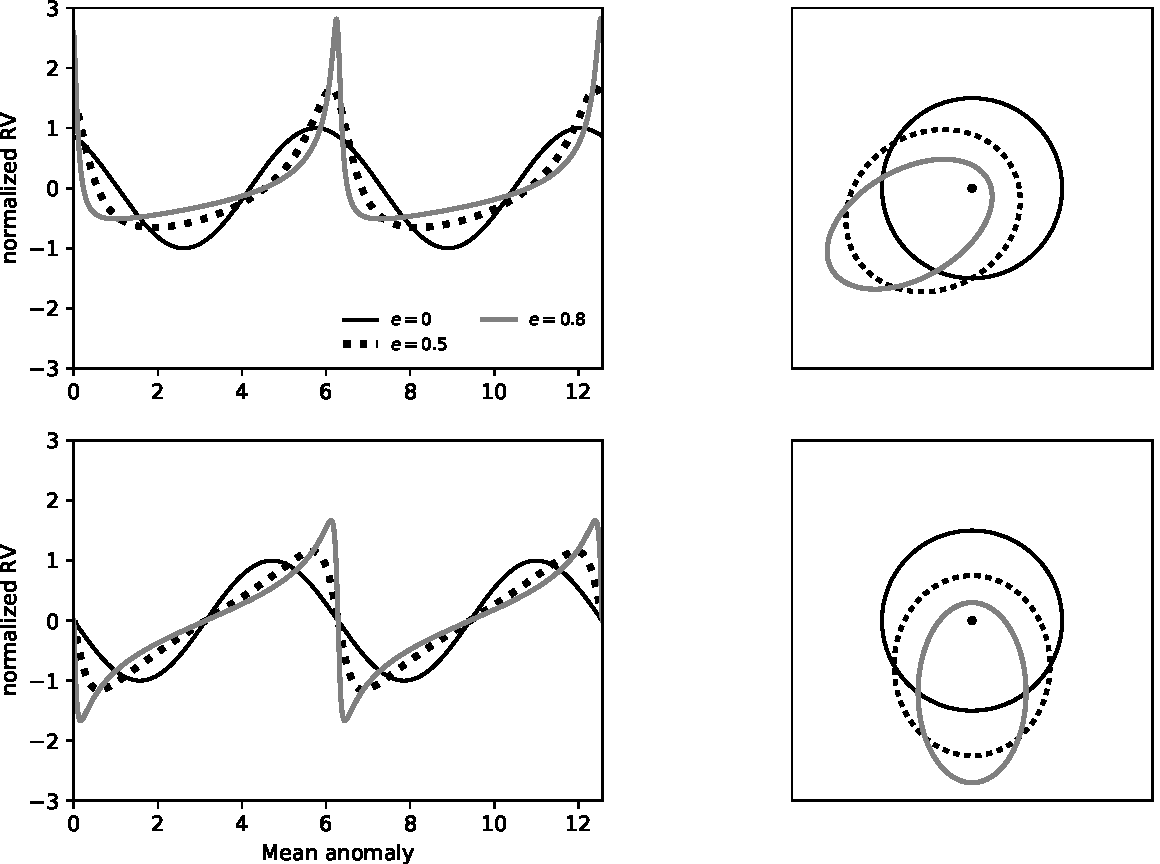
\includegraphics[width=\linewidth]{fig/rvsim.pdf}
\end{center}
	\caption{視線速度カーブ(左)と対応する軌道(右)。上段は$\omega=\pi/6$,下段は$\omega=\pi/2$である。線種は黒実線が$e=0$、黒点線が$e=0.5$、灰色実線が$e=0.8$に対応している。右の楕円は$i=\pi/2$の時に軌道を上から見たものに対応し、下から上むきに視線方向をとると、視線速度カーブの恒星軌道、上から下向きにとると惑星の軌道に対応する。\label{fig:rvsim}}	
\end{figure} 


\begin{itembox}{Binary Mass Function$\,^\dagger$}
%\tiny
\footnotesize
\color{gray}
そもそも視線速度解析は恒星惑星系以前に連星系で発展してきた。この場合、$M_p \ll M_\star$は成り立たない。式(\ref{eq:vrKrv})を、$\star \to 1$と$p \to 2$で書き直し、ケプラー第三法則(\ref{eq:kep3})を用いて、右辺に観測量だけ、左辺に物理パラメタとわけて書くと
\begin{align}
  \label{eq:bmfunc}
  f \equiv \frac{M_2^3}{(M_1 + M_2)^2} \sin^3{i} = \frac{P K_1^3}{2 \pi G} (1 - e^2)^{3/2}
\end{align}
のようになる。この$f$が、一般の質量比の場合、星1の視線速度カーブの観測量$K_1$、$e$、$P$のみからわかる量である。この$f$をbinary mass function\index{Binary Mass Function@Binary Mass Function}と呼ぶ。

また、逆に
\begin{align}
  \label{eq:semiamp2}
  K_1 &= 29.8 \, [\mathrm{km/s}]  \frac{\sin{i}}{\sqrt{1 - e^2}} \left( \frac{M_2}{M_1 + M_2} \right) \nonumber \\
  &\times \left( \frac{M_1 + M_2}{M_\odot} \right)^{1/3} \left( \frac{P}{1 \mathrm{yr}} \right)^{1/3}
\end{align}
とスケーリングされた式を用いると、連星系の場合の検出可能性の見積もりに便利である。この29.8 km/sという値は地球の公転速度に一致している。

\end{itembox}

\section{アストロメトリ}
視線速度変動は3次元ケプラー運動の$\dot{Z}$成分の運動情報を用いていた。アストロメトリは天球上の星の位置を計測する手法であるから、($X$,$Y$)成分の運動情報を用いることになる。固有運動・パララックスを補正後の二体運動による恒星の位置は、観測者から恒星までの距離を$d$として、観測量である角度(離角)としてあらわすと
\begin{align}
   {\boldsymbol{\theta}} = \frac{\hat{\rv}_\star}{d} = - \frac{M_p}{M_\star + M_p} \frac{\hat{\rv}}{d}
\end{align}
に二次元射影となる。すなわち式(\ref{eq:threed})より、
\begin{align}
    \theta_x &= - \frac{M_p}{M_\star + M_p} \frac{X}{d} = - \frac{M_p}{M_\star + M_p} \frac{r}{d} \nonumber\\
    &\times [\cos\!\bigl(f+\omega\bigr)\cos\Omega
 - \sin\!\bigl(f+\omega\bigr)\cos i\,\sin\Omega]\\
     \theta_y &= - \frac{M_p}{M_\star + M_p} \frac{Y}{d} =- \frac{M_p}{M_\star + M_p}\frac{r}{d} \nonumber\\
     &\times [ \cos\!\bigl(f+\omega\bigr)\sin\Omega
 + \sin\!\bigl(f+\omega\bigr)\cos i\,\cos\Omega]
\end{align}
となる。この解は($i \to \pi - i$, $f \to 2 \pi - f$, $\omega \to 2 \pi - \omega$)の変換に不変であり、これはアストロメトリのみでは惑星が近づいているのか遠ざかっているのかはわからない。
